%!TEX root = ../../super_main.tex

\section{Snapshot}
\label{sec:snapshot}

% Motivation 
We will also need a model for the gathered data to complement the specifications of how the individual snapshots should be composed. This model should be able handle different types of data from different sensors. Some measurements will be simple floating point numbers, to approximate real numbers, and others will consist of more complex types aggregating different values possibly of different types.  

\section{Compression of Floats}
As described in \secref{sec:start_configuration}, we would like to minimize the power consumption of our application. To do this, we minimize the footprint of the collected data when transmitting it wirelessly, since this is very expensive. To do this, we compress values gathered from sensors. Most sensors will make measurements described by three \mono{float} values. We designed a class called \mono{FloatTripleMeasurement} which is used to compress these three values a single \mono{long}, meaning we convert $12$ bytes ($3 \times 4$ bytes) to be stored in $8$ bytes. We do this by sacrificing some of the precision of a regular float.
\\\\
When compressing, we assume that the integer part does not exceed $7$ numbers. We do this because the sensors only produce values ranging from $-360$ to $360$. We strip the decimal separator from the floats an treat them as a $20$ bit integer value, where the first bit determines whether the value is positive or negative. This means that we now use $60$ bits for storing the compressed value of the floats. We use the remainder of the long to add 3 bits for representing where the decimal should be placed. A visualization of the method used to compress floats can be seen in \figref{fig:float_triple_convert} and \figref{fig:float_triple_bit} respectively.
\begin{figure}[!htbp]
    \begin{alignat*}{6}
       &8.138   &&                   &&   && 8138  &&                   && \text{\mono{00000001111111001010}} \\
      -&12.821  && ~~ \rightarrow ~~ && - && 12821 && ~~ \rightarrow ~~ && \text{\mono{10000011001000010101}} \\
       &42.4878 &&                   &&   && 42487 &&                   && \text{\mono{00001010010111110111}} 
    \end{alignat*}
    \caption{Compression of floats.}
    \label{fig:float_triple_convert}
\end{figure}

\begin{figure}[!htbp]
    \centering
    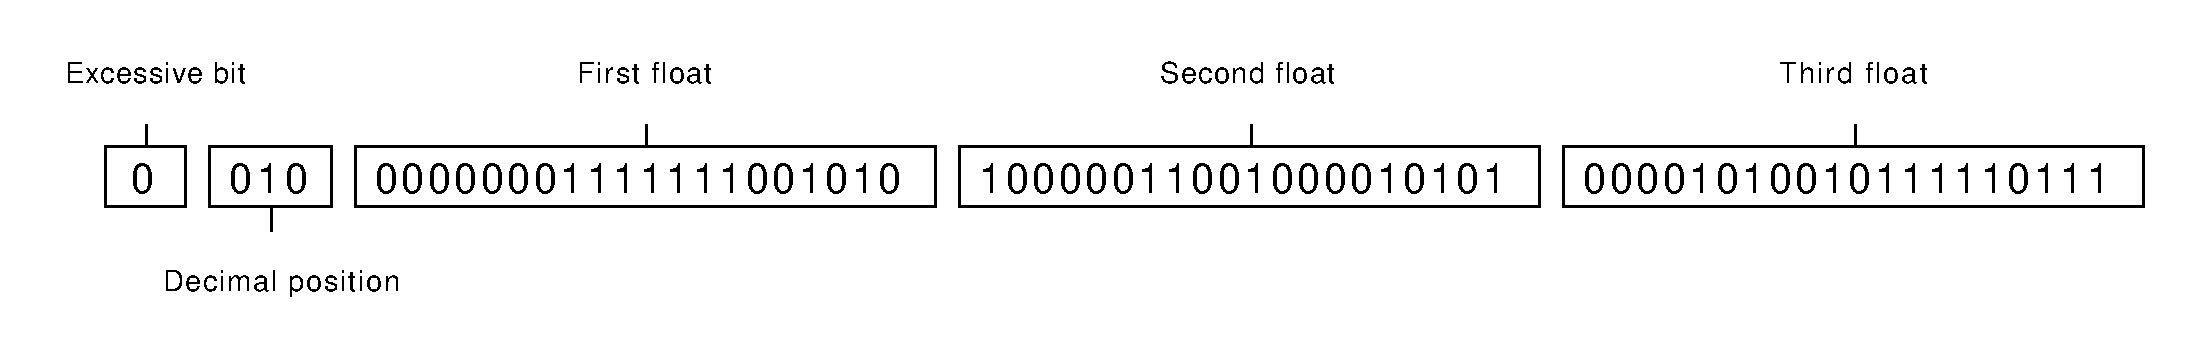
\includegraphics[width=\textwidth]{graphic/data_modeling/float_triple_bit.pdf}
    \caption{The bit representation of a FloatTriple.}
    \label{fig:float_triple_bit}
\end{figure}

We wanted to compress the floating point values of the sensors so that the size of the data we need to send over network and store on the device would decrease. However, this compression does not come for free. We actively make a trade off between size of data stored and CPU cycles used for compressing and decompressing the values.  
\todo[inline]{Insert test af performance}